\documentclass[sigchi]{acmart}

\def\tightlist{}
\settopmatter{printacmref=false}
\renewcommand\footnotetextcopyrightpermission[1]{}
\settopmatter{printfolios=true}

\usepackage{color}
\usepackage{fancyvrb}
\newcommand{\VerbBar}{|}
\newcommand{\VERB}{\Verb[commandchars=\\\{\}]}
\DefineVerbatimEnvironment{Highlighting}{Verbatim}{commandchars=\\\{\}}
% Add ',fontsize=\small' for more characters per line
\usepackage{framed}
\definecolor{shadecolor}{RGB}{248,248,248}
\newenvironment{Shaded}{\begin{snugshade}}{\end{snugshade}}
\newcommand{\AlertTok}[1]{\textcolor[rgb]{0.94,0.16,0.16}{#1}}
\newcommand{\AnnotationTok}[1]{\textcolor[rgb]{0.56,0.35,0.01}{\textbf{\textit{#1}}}}
\newcommand{\AttributeTok}[1]{\textcolor[rgb]{0.77,0.63,0.00}{#1}}
\newcommand{\BaseNTok}[1]{\textcolor[rgb]{0.00,0.00,0.81}{#1}}
\newcommand{\BuiltInTok}[1]{#1}
\newcommand{\CharTok}[1]{\textcolor[rgb]{0.31,0.60,0.02}{#1}}
\newcommand{\CommentTok}[1]{\textcolor[rgb]{0.56,0.35,0.01}{\textit{#1}}}
\newcommand{\CommentVarTok}[1]{\textcolor[rgb]{0.56,0.35,0.01}{\textbf{\textit{#1}}}}
\newcommand{\ConstantTok}[1]{\textcolor[rgb]{0.00,0.00,0.00}{#1}}
\newcommand{\ControlFlowTok}[1]{\textcolor[rgb]{0.13,0.29,0.53}{\textbf{#1}}}
\newcommand{\DataTypeTok}[1]{\textcolor[rgb]{0.13,0.29,0.53}{#1}}
\newcommand{\DecValTok}[1]{\textcolor[rgb]{0.00,0.00,0.81}{#1}}
\newcommand{\DocumentationTok}[1]{\textcolor[rgb]{0.56,0.35,0.01}{\textbf{\textit{#1}}}}
\newcommand{\ErrorTok}[1]{\textcolor[rgb]{0.64,0.00,0.00}{\textbf{#1}}}
\newcommand{\ExtensionTok}[1]{#1}
\newcommand{\FloatTok}[1]{\textcolor[rgb]{0.00,0.00,0.81}{#1}}
\newcommand{\FunctionTok}[1]{\textcolor[rgb]{0.00,0.00,0.00}{#1}}
\newcommand{\ImportTok}[1]{#1}
\newcommand{\InformationTok}[1]{\textcolor[rgb]{0.56,0.35,0.01}{\textbf{\textit{#1}}}}
\newcommand{\KeywordTok}[1]{\textcolor[rgb]{0.13,0.29,0.53}{\textbf{#1}}}
\newcommand{\NormalTok}[1]{#1}
\newcommand{\OperatorTok}[1]{\textcolor[rgb]{0.81,0.36,0.00}{\textbf{#1}}}
\newcommand{\OtherTok}[1]{\textcolor[rgb]{0.56,0.35,0.01}{#1}}
\newcommand{\PreprocessorTok}[1]{\textcolor[rgb]{0.56,0.35,0.01}{\textit{#1}}}
\newcommand{\RegionMarkerTok}[1]{#1}
\newcommand{\SpecialCharTok}[1]{\textcolor[rgb]{0.00,0.00,0.00}{#1}}
\newcommand{\SpecialStringTok}[1]{\textcolor[rgb]{0.31,0.60,0.02}{#1}}
\newcommand{\StringTok}[1]{\textcolor[rgb]{0.31,0.60,0.02}{#1}}
\newcommand{\VariableTok}[1]{\textcolor[rgb]{0.00,0.00,0.00}{#1}}
\newcommand{\VerbatimStringTok}[1]{\textcolor[rgb]{0.31,0.60,0.02}{#1}}
\newcommand{\WarningTok}[1]{\textcolor[rgb]{0.56,0.35,0.01}{\textbf{\textit{#1}}}}

\usepackage{booktabs} % For formal tables

% Copyright
\setcopyright{none}
%\setcopyright{acmcopyright}
%\setcopyright{acmlicensed}
%\setcopyright{rightsretained}
%\setcopyright{usgov}
%\setcopyright{usgovmixed}
%\setcopyright{cagov}
%\setcopyright{licensedcagov}
%\setcopyright{cagovmixed}
%\setcopyright{licensedothergov}

% DOI
\acmDOI{10.475/123_4}

% ISBN
\acmISBN{123-4567-24-567/08/06}

%Conference
\acmConference[Business Intelligence]{Assignment 3}{January 2021}{Linz/Vienna, Austria}
\acmYear{2021}
\copyrightyear{2021}

\acmPrice{15.00}


\begin{document}
\title{Predicting the resale value of used cars}
\subtitle{Created using R Markdown}

\author{Simone Andreetto}
\affiliation{%
  \institution{01635069}
}

\author{Felix Winterleitner}
\affiliation{%
  \institution{01612776}
}

% The default list of authors is too long for headers.
\renewcommand{\shortauthors}{S. Andreetto et al.}


\begin{abstract}
This is Assignment 3 in Business Intelligence @ TU Wien in the winter term of 2020.
\end{abstract}


\keywords{Business Intelligence, R, Rmd, Spark}

\begin{teaserfigure}
  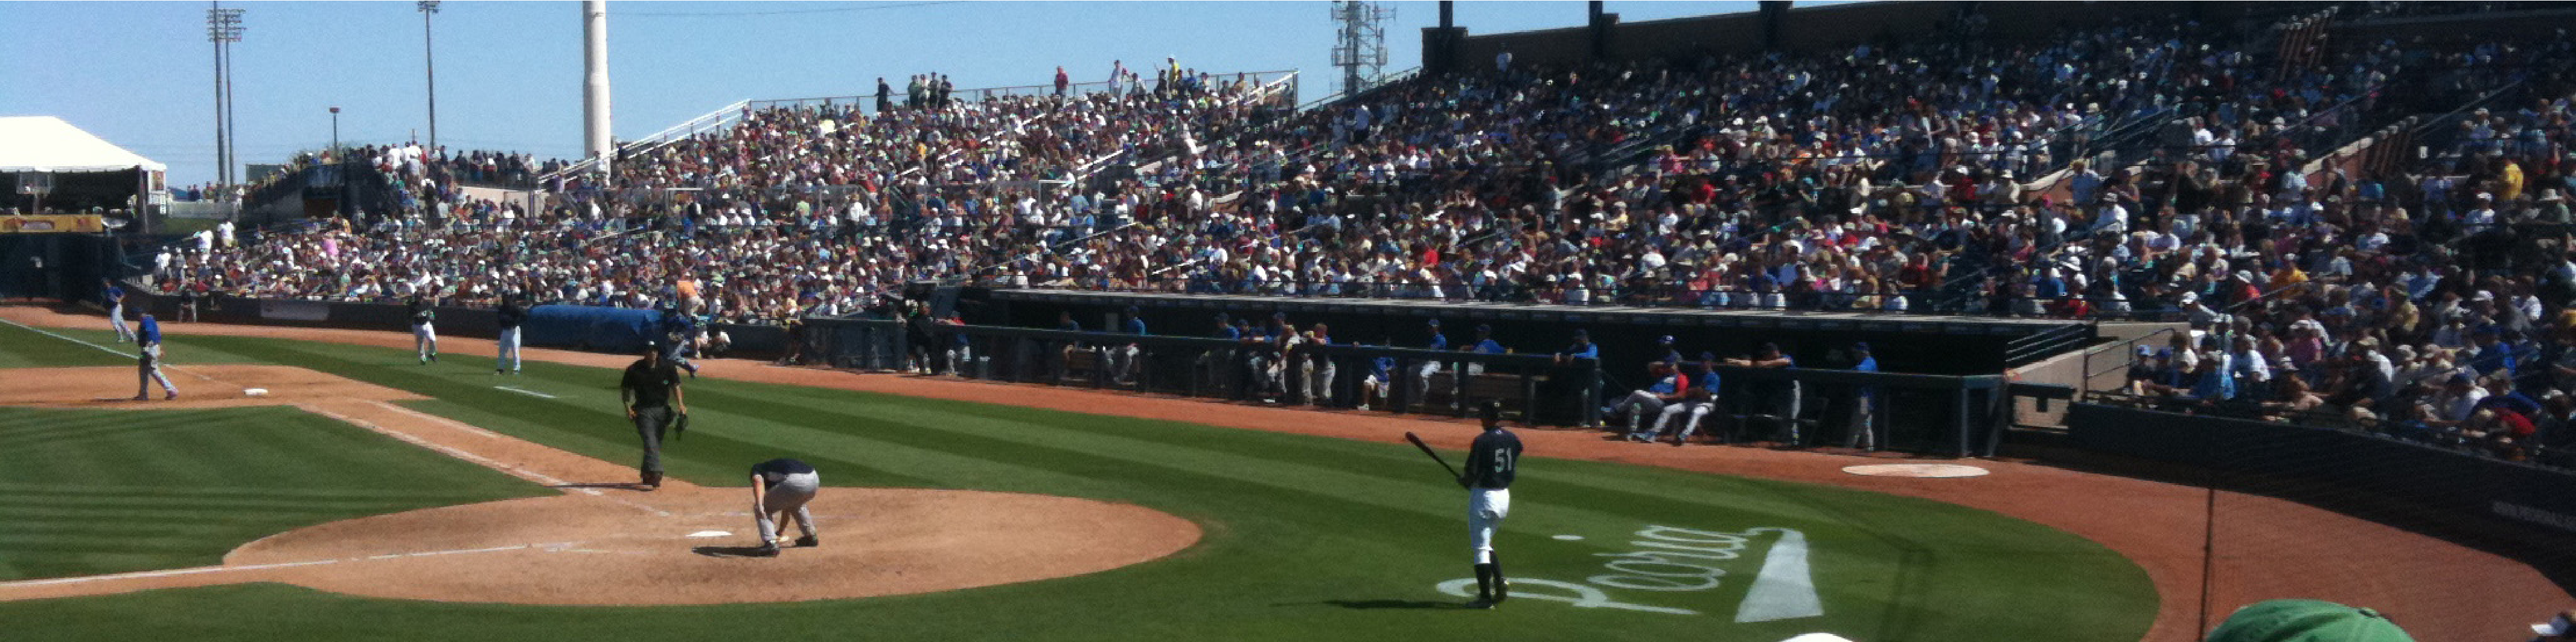
\includegraphics[width=\textwidth]{sampleteaser}
  \caption{This is a teaser}
  \label{fig:teaser}
\end{teaserfigure}


\maketitle

\hypertarget{introduction}{%
\section{Introduction}\label{introduction}}

For this project, we used a dataset found on Kaggle.com provided by user Aditya \citep{Aditya}. It contains a collection of different used car listings obtained by searching through online marketplaces using a web scraper. The dataset is split into different files, one per car brand. The brands for which data is available are:

\begin{itemize}
\tightlist
\item
  Audi
\item
  BMW
\item
  Ford
\item
  Hyundai
\item
  Mercedes
\item
  Skoda
\item
  Toyota
\item
  Vauxhall (= Opel in Great Britain)
\item
  VW
\end{itemize}

Additionally, the data set contains files with premade subsets of above mentioned car brands, for example \emph{cclass.csv}, which contains only listings for the Mercedes model C Class. We chose to only utilize the unfiltered datasets.

Apart from the car brand, there are a number of other attributes available for each data entry.

\begin{itemize}
\tightlist
\item
  car model
\item
  year of first registration
\item
  transmission type
\item
  mileage
\item
  fuel type
\item
  tax
\item
  miles per gallon of fuel
\item
  engine size
\end{itemize}

as well as the target variable price.

\hypertarget{business-understanding}{%
\section{Business Understanding}\label{business-understanding}}

\hypertarget{a.-scenario}{%
\subsection{a. Scenario}\label{a.-scenario}}

A group of entrepreneurs in the used car business want to counteract the ongoing trend of people selling their cars to other private individuals directly without involving commercial reseller, which has become very easy given the availability of online market places for used goods. The idea is the following: Customers are offered a new web-based platform where they can enter the most important key facts about the car they would like to sell. The platform immediately returns a first estimate of the price the platform owners would pay for the car. This estimate should be based on a model created from the used car listing data available.

\hypertarget{b.-business-objectives}{%
\subsection{b. Business Objectives}\label{b.-business-objectives}}

The business objectives is in short:

\textbf{What is the expected value of a used car based on the given data entries?}

Answering this question helps the platform in multiple ways.

\begin{itemize}
\tightlist
\item
  make it more convenient for customers to sell their used car by getting an accurate first estimate right after entering the data
\item
  increase revenues by missing out on fewer chances to buy used cars (more cars resold via the platform instead of directly to other buyers)
\item
  speed up final evaluation of car value by offering a good starting point
\item
  base offers made to customers on true market values
\end{itemize}

\hypertarget{c.-business-success-criteria}{%
\subsection{c. Business Success Criteria}\label{c.-business-success-criteria}}

The following criteria need to be met by the prediction:

\begin{itemize}
\item
  The estimate should lead to a conversion rate of more than 30\%, meaning that at least 30\% of the users that enter their car data on the website actually proceed to sell their car on the platform.
\item
  The estimations should never lead to an effective loss for the company. Therefore, estimations that are too high need to be avoided.
\end{itemize}

\hypertarget{d.-data-mining-goals}{%
\subsection{d. Data Mining Goals}\label{d.-data-mining-goals}}

In order to fulfill the business objective of determining an accurate price estimate, a regression problem needs to be solved. The input data consists of the 9 attributes mentioned above.

\hypertarget{e.-data-mining-success-criteria}{%
\subsection{e. Data Mining Success Criteria}\label{e.-data-mining-success-criteria}}

Regarding the result of the estimation, one important success criterion is:

\begin{itemize}
\tightlist
\item
  The estimate needs to be within a range of the actual price +/- 15\% for 95\% of the estimations made.
\end{itemize}

This is important because estimates that are further off the actual price may lead to:

\begin{itemize}
\tightlist
\item
  People aborting the process when the estimate is much lower than their expectation
\item
  People entering the negotiations with far inflated expectation, effectively reducing the changes of the platform owners to score a good deal
\end{itemize}

\hypertarget{data-understanding}{%
\section{Data Understanding}\label{data-understanding}}

In the following section, a data description report containing data types, statistical properties, data quality aspects as well as a visual exploration of data properties is presented.

\hypertarget{a.-data-types}{%
\subsection{a. Data Types}\label{a.-data-types}}

The attributes in the data set have the data types shown in \textbf{Table \ref{tab:table-datatypes}.}

\begin{table}

\caption{\label{tab:table-datatypes}Data Types of the source data}
\centering
\begin{tabular}[t]{ll}
\toprule
Attribute & Type\\
\midrule
model & String, nominal\\
age & Integer, interval\\
year & Integer, ratio\\
transmission & String, nominal\\
mileage & Integer, ratio\\
\addlinespace
fuelType & String, nominal\\
tax & Integer, ratio\\
mpg & Float, ratio\\
engineSize & Float, ratio\\
price & Integer, ratio\\
\bottomrule
\end{tabular}
\end{table}

\hypertarget{b.-statistical-properties}{%
\subsection{b. Statistical Properties}\label{b.-statistical-properties}}

\begin{Shaded}
\begin{Highlighting}[]
\KeywordTok{options}\NormalTok{(}\DataTypeTok{width =} \DecValTok{60}\NormalTok{)}
\KeywordTok{summary}\NormalTok{(car_data)}
\end{Highlighting}
\end{Shaded}

\begin{verbatim}
##     brand              model                year     
##  Length:99187       Length:99187       Min.   :1970  
##  Class :character   Class :character   1st Qu.:2016  
##  Mode  :character   Mode  :character   Median :2017  
##                                        Mean   :2017  
##                                        3rd Qu.:2019  
##                                        Max.   :2060  
##  transmission          mileage         fuelType        
##  Length:99187       Min.   :     1   Length:99187      
##  Class :character   1st Qu.:  7425   Class :character  
##  Mode  :character   Median : 17460   Mode  :character  
##                     Mean   : 23059                     
##                     3rd Qu.: 32339                     
##                     Max.   :323000                     
##       tax             mpg           engineSize   
##  Min.   :  0.0   Min.   :  0.30   Min.   :0.000  
##  1st Qu.:125.0   1st Qu.: 47.10   1st Qu.:1.200  
##  Median :145.0   Median : 54.30   Median :1.600  
##  Mean   :120.3   Mean   : 55.17   Mean   :1.663  
##  3rd Qu.:145.0   3rd Qu.: 62.80   3rd Qu.:2.000  
##  Max.   :580.0   Max.   :470.80   Max.   :6.600  
##      price             age         
##  Min.   :   450   Min.   :-40.000  
##  1st Qu.:  9999   1st Qu.:  1.000  
##  Median : 14495   Median :  3.000  
##  Mean   : 16805   Mean   :  2.912  
##  3rd Qu.: 20870   3rd Qu.:  4.000  
##  Max.   :159999   Max.   : 50.000
\end{verbatim}

\hypertarget{c.-data-quality-aspects}{%
\subsection{c. Data Quality aspects}\label{c.-data-quality-aspects}}

Since the data is recorded from the internet there is the possibility of it containing invalid information or missing values.

To begin with, we check the data for missing values. However, in this speficic case, there are none.

\begin{Shaded}
\begin{Highlighting}[]
\KeywordTok{dim}\NormalTok{(car_data) }\OperatorTok{==}
\StringTok{  }\KeywordTok{dim}\NormalTok{(car_data[}\KeywordTok{complete.cases}\NormalTok{(car_data),])}
\end{Highlighting}
\end{Shaded}

\begin{verbatim}
## [1] TRUE TRUE
\end{verbatim}

Next up, we check plausibility of some of the extreme cases of numerical values. To keep it short, we only included one exemplary output her and then summarize the findings.

\begin{Shaded}
\begin{Highlighting}[]
\KeywordTok{options}\NormalTok{(}\DataTypeTok{width =} \DecValTok{60}\NormalTok{)}
\KeywordTok{head}\NormalTok{(car_data[}\KeywordTok{order}\NormalTok{(car_data}\OperatorTok{$}\NormalTok{age),], }\DecValTok{5}\NormalTok{)}
\end{Highlighting}
\end{Shaded}

\begin{verbatim}
## # A tibble: 5 x 11
##   brand model  year transmission mileage fuelType   tax
##   <chr> <chr> <dbl> <chr>          <dbl> <chr>    <dbl>
## 1 Ford  Fies~  2060 Automatic      54807 Petrol     205
## 2 Audi  Q7     2020 Semi-Auto         10 Diesel     145
## 3 Audi  Q5     2020 Semi-Auto         10 Petrol     145
## 4 Audi  Q5     2020 Semi-Auto         10 Petrol     145
## 5 Audi  A4     2020 Semi-Auto         10 Petrol     145
## # ... with 4 more variables: mpg <dbl>, engineSize <dbl>,
## #   price <dbl>, age <dbl>
\end{verbatim}

\begin{Shaded}
\begin{Highlighting}[]
\CommentTok{# year 2060 is an error}

\KeywordTok{head}\NormalTok{(car_data[}\KeywordTok{order}\NormalTok{(}\OperatorTok{-}\NormalTok{car_data}\OperatorTok{$}\NormalTok{age),], }\DecValTok{5}\NormalTok{)}
\end{Highlighting}
\end{Shaded}

\begin{verbatim}
## # A tibble: 5 x 11
##   brand model  year transmission mileage fuelType   tax
##   <chr> <chr> <dbl> <chr>          <dbl> <chr>    <dbl>
## 1 Merc~ M Cl~  1970 Automatic      14000 Diesel     305
## 2 Vaux~ Zafi~  1970 Manual         37357 Petrol     200
## 3 BMW   5 Se~  1996 Automatic      36000 Petrol     270
## 4 Ford  Esco~  1996 Manual         50000 Petrol     265
## 5 Audi  A8     1997 Automatic     122000 Petrol     265
## # ... with 4 more variables: mpg <dbl>, engineSize <dbl>,
## #   price <dbl>, age <dbl>
\end{verbatim}

\begin{Shaded}
\begin{Highlighting}[]
\CommentTok{# the oldest cars seem realistic}
\end{Highlighting}
\end{Shaded}

Most of the extreme values in the dataset were realistic. Some entries contain questionable combinations of age and mileage, unrealistically high or low MPG values or ``0'' engine sizes. In those cases, some filtering should be done.

\hypertarget{d.-visual-exploration-of-data-properties-and-hypotheses}{%
\subsection{d. Visual Exploration of data properties and hypotheses}\label{d.-visual-exploration-of-data-properties-and-hypotheses}}

In the following figures, boxplots illustrate the ranges of the numeric (ratio) variables.

\begin{figure*}
\includegraphics[width=0.98\textwidth]{step6_files/figure-latex/figure-boxplots-1} \caption{Boxplots on the distribution of the numeric attributes}\label{fig:figure-boxplots}
\end{figure*}

There are a few things we can learn from these diagrams. For example, it is interesting to see car listings contained in the data set are mostly for rather new cars, with a mileage median of less than 25000 miles. Taking a look at \textbf{Figure \ref{fig:car-age}}, this suspicion is confirmed. The vast majority of cars in the dataset is indeed less than five years old. There is 1 entry where the cars year is seemingly bigger than 2020, that is 2060, which will have to be dealt with in later steps.

\begin{figure}
\includegraphics[width=0.98\columnwidth]{step6_files/figure-latex/car-age-1} \caption{Histogram of car age.}\label{fig:car-age}
\end{figure}

The correlation plot in \textbf{Figure \ref{fig:correlationmatrix}} shows some pretty good correlation between ther predictor variables and the price, so we might be able to create a solid regression using the data available.

\begin{figure}
\includegraphics[width=0.98\columnwidth]{step6_files/figure-latex/correlationmatrix-1} \caption{Pairs of all numeric attributes}\label{fig:correlationmatrix}
\end{figure}

From the view point of a human estimating the value of a used car, the most influential attributes should be age, mileage and brand/model as well as general condition, which is however not part of our dataset. Looking at the correlation matrix, we see that there is indeed a significant correlation between price and age as well as mileage. For model and brand, the correlation is much lower.

\hypertarget{data-preparation-report}{%
\section{Data Preparation report}\label{data-preparation-report}}

Insert content here.

\begin{enumerate}
\def\labelenumi{\alph{enumi}.}
\tightlist
\item
  Analyze options and potential for derived attributes (note: if the potential is considered low, these obviously do not necessarily have to be applied for your analysis, but options should be documented)
\item
  Analyze options for additional external data sources, attributes that might be useful to better address the business objectives or data mining goals (Note: this description may be hypothetical, i.e.~you are not necessarily required to actually obtain and integrate the external data for the analysis)
\end{enumerate}

\hypertarget{e.g.car-horse-power}{%
\paragraph{e.g.~Car Horse Power}\label{e.g.car-horse-power}}

\begin{enumerate}
\def\labelenumi{\alph{enumi}.}
\setcounter{enumi}{2}
\tightlist
\item
  Describe other pre-processing steps considered, specifying which ones were applied or not applied due to which reason. (e.g.~data cleansing, transformations, binning, scaling, outlier removal, attribute removal, transcoding, \ldots{}) at a level of detail that ensures reproducibility of changes to the data. (Code may be supplied as supplement to the submission in case you produce your own code)
\end{enumerate}

\hypertarget{modeling}{%
\section{Modeling}\label{modeling}}

\begin{enumerate}
\def\labelenumi{\alph{enumi}.}
\tightlist
\item
  Identify suitable data mining algorithms and select one of these as the most suitable for your experiments, providing a brief justification.
\end{enumerate}

The goal is to estimate the price for a car based on it inputed characteristics based on the training data containing nine attributes as well as the prediction lable. Therefore it is a supervised learning with regression, prediction of a numerical value.

When choosing the a regression model it has to deliver sufficient results, while being efficient in computation.
While complex regression models might deliver higher accuracies, they easily become difficult to interpret and follow back decisions.
Generalized linear regression is the got to regression model as it is fast to train and delivers good estimates and predictions. It's computational requirements depending on the data are managable.

\begin{enumerate}
\def\labelenumi{\alph{enumi}.}
\setcounter{enumi}{1}
\tightlist
\item
  Identify the hyper-parameters available for tuning in your chosen algorithm and select one that you deem most relevant for tuning, providing a brief justification.
\end{enumerate}

Choosing a linear regression model leaves open the possibility to modify the formula to reproduce a linear relationship between the attributes and the predicted value. While doing it manually is very timeintensive and inefficient it can be implemented with the use of Generalized additive models (gam). This model allows to apply smoothing functions on the single parameters to improve prediction outcome. Effectively combining generalized linear models with additive models.

\begin{enumerate}
\def\labelenumi{\alph{enumi}.}
\setcounter{enumi}{2}
\tightlist
\item
  Define and document a train / validation / test set split, considering where necessary appropriate stratification, any dependencies between data instances (e.g.~time series data) and relative sizes of the respective subsets.
\end{enumerate}

Dividin the data train, validation and test set. In the ratio:
* train: 70\%
* validate: 15\%
* test: 15\%

To ensure rproducability a seed is set.

\begin{Shaded}
\begin{Highlighting}[]
\KeywordTok{set.seed}\NormalTok{(}\DecValTok{1}\NormalTok{)}
\NormalTok{assignment <-}\StringTok{ }\KeywordTok{sample}\NormalTok{(}\DecValTok{1}\OperatorTok{:}\DecValTok{3}\NormalTok{,}\KeywordTok{nrow}\NormalTok{(car_data),}\DataTypeTok{prob =} \KeywordTok{c}\NormalTok{(}\FloatTok{0.7}\NormalTok{,}\FloatTok{0.15}\NormalTok{,}\FloatTok{0.15}\NormalTok{), }\DataTypeTok{replace =} \OtherTok{TRUE}\NormalTok{)}

\NormalTok{train_data <-}\StringTok{ }\NormalTok{car_data[assignment}\OperatorTok{==}\DecValTok{1}\NormalTok{,]}
\NormalTok{test_data <-}\StringTok{ }\NormalTok{car_data[assignment}\OperatorTok{==}\DecValTok{2}\NormalTok{,]}
\NormalTok{validate_data <-}\StringTok{ }\NormalTok{car_data[assignment}\OperatorTok{==}\DecValTok{3}\NormalTok{,]}
\end{Highlighting}
\end{Shaded}

Splitting the data in train, test and validate samples, caused failuers in the prediciton process, as some car models are very scarse or unique. Meaning the case happened of certain models appearing only in the testing or validating samples and therefore being unknown levels to the model. To resolve this issue, new levels (car models not present in the training sample) were removed from the testing and validation sample.
Further thoughtprocess on this matter in regards of usability in business are present in \textbf{ADD REFERENCE HERE!}

\begin{Shaded}
\begin{Highlighting}[]
\CommentTok{# Analysing data on the carmodels}
\KeywordTok{barplot}\NormalTok{(}\KeywordTok{prop.table}\NormalTok{(}\KeywordTok{table}\NormalTok{(car_data}\OperatorTok{$}\NormalTok{model)))}
\end{Highlighting}
\end{Shaded}

\includegraphics[width=0.98\columnwidth]{step6_files/figure-latex/unnamed-chunk-7-1}

\begin{Shaded}
\begin{Highlighting}[]
\KeywordTok{head}\NormalTok{(}\KeywordTok{sort}\NormalTok{(}\KeywordTok{table}\NormalTok{(car_data}\OperatorTok{$}\NormalTok{model),}\DataTypeTok{decreasing =} \OtherTok{TRUE}\NormalTok{),}\DecValTok{5}\NormalTok{)}
\end{Highlighting}
\end{Shaded}

\begin{verbatim}
## 
##  Fiesta    Golf   Focus C Class   Corsa 
##    6557    4863    4588    3747    3441
\end{verbatim}

\begin{Shaded}
\begin{Highlighting}[]
\KeywordTok{tail}\NormalTok{(}\KeywordTok{sort}\NormalTok{(}\KeywordTok{table}\NormalTok{(car_data}\OperatorTok{$}\NormalTok{model),}\DataTypeTok{decreasing =} \OtherTok{TRUE}\NormalTok{),}\DecValTok{5}\NormalTok{)}
\end{Highlighting}
\end{Shaded}

\begin{verbatim}
## 
##           Amica          Escort          Ranger 
##               1               1               1 
##             RS7 Transit Tourneo 
##               1               1
\end{verbatim}

\begin{Shaded}
\begin{Highlighting}[]
\CommentTok{# reveals that some carmodels are only present once in the datamodel}

\CommentTok{# Carmodels missing in the trainingdata}
\NormalTok{missing_fact_test <-}\StringTok{ }\KeywordTok{setdiff}\NormalTok{(}\KeywordTok{unique}\NormalTok{(test_data}\OperatorTok{$}\NormalTok{model), }\KeywordTok{unique}\NormalTok{(train_data}\OperatorTok{$}\NormalTok{model))}
\NormalTok{missing_fact_validate <-}\StringTok{ }\KeywordTok{setdiff}\NormalTok{(}\KeywordTok{unique}\NormalTok{(validate_data}\OperatorTok{$}\NormalTok{model), }\KeywordTok{unique}\NormalTok{(train_data}\OperatorTok{$}\NormalTok{model))}

\NormalTok{cleaned_test_data <-}\StringTok{ }\NormalTok{test_data[}\OperatorTok{!}\NormalTok{test_data}\OperatorTok{$}\NormalTok{model }\OperatorTok\StringTok{ }\NormalTok{missing_fact_test,]}
\NormalTok{cleaned_validate_data <-}\StringTok{ }\NormalTok{validate_data[}\OperatorTok{!}\NormalTok{validate_data}\OperatorTok{$}\NormalTok{model }\OperatorTok\StringTok{ }\NormalTok{missing_fact_validate,]}
\end{Highlighting}
\end{Shaded}

\begin{enumerate}
\def\labelenumi{\alph{enumi}.}
\setcounter{enumi}{3}
\item
  Train the model on the training set and comparing the performance on the validation set to identify the best hyper-parameter setting, explicitly documenting all parameter settings (avoid stating simply to have used ``default parameters'', focus on reproducibility of the results you report).
\item
  Report suitable performance metrics supported, where possible, by figures/graphs showing the tuning process of the hyper parameter.
\end{enumerate}

\begin{Shaded}
\begin{Highlighting}[]
\CommentTok{# summary}
\KeywordTok{summary}\NormalTok{(glm_model)}\OperatorTok{$}\NormalTok{r.squared}
\end{Highlighting}
\end{Shaded}

\begin{verbatim}
## [1] 0.866457
\end{verbatim}

\begin{Shaded}
\begin{Highlighting}[]
\KeywordTok{summary}\NormalTok{(gam_model)}\OperatorTok{$}\NormalTok{r.sq}
\end{Highlighting}
\end{Shaded}

\begin{verbatim}
## [1] 0.9018316
\end{verbatim}

\begin{Shaded}
\begin{Highlighting}[]
\KeywordTok{plot}\NormalTok{(cleaned_test_data}\OperatorTok{$}\NormalTok{price,glm_pred)}
\end{Highlighting}
\end{Shaded}

\includegraphics{step6_files/figure-latex/unnamed-chunk-10-1.pdf}

\begin{Shaded}
\begin{Highlighting}[]
\KeywordTok{plot}\NormalTok{(cleaned_test_data}\OperatorTok{$}\NormalTok{price,gam_pred)}
\end{Highlighting}
\end{Shaded}

\includegraphics{step6_files/figure-latex/unnamed-chunk-10-2.pdf}

\begin{Shaded}
\begin{Highlighting}[]
\KeywordTok{hist}\NormalTok{(cleaned_test_data}\OperatorTok{$}\NormalTok{price}\OperatorTok{-}\NormalTok{glm_pred,}\DataTypeTok{breaks =} \DecValTok{200}\NormalTok{)}
\end{Highlighting}
\end{Shaded}

\includegraphics{step6_files/figure-latex/unnamed-chunk-10-3.pdf}

\begin{Shaded}
\begin{Highlighting}[]
\KeywordTok{hist}\NormalTok{(cleaned_test_data}\OperatorTok{$}\NormalTok{price}\OperatorTok{-}\NormalTok{gam_pred,}\DataTypeTok{breaks =} \DecValTok{200}\NormalTok{)}
\end{Highlighting}
\end{Shaded}

\includegraphics{step6_files/figure-latex/unnamed-chunk-10-4.pdf}

\begin{Shaded}
\begin{Highlighting}[]
\KeywordTok{mean}\NormalTok{(}\KeywordTok{abs}\NormalTok{((cleaned_test_data}\OperatorTok{$}\NormalTok{price }\OperatorTok{-}\StringTok{ }\NormalTok{glm_pred)}\OperatorTok{/}\NormalTok{cleaned_test_data}\OperatorTok{$}\NormalTok{price))}
\end{Highlighting}
\end{Shaded}

\begin{verbatim}
## [1] 0.1768322
\end{verbatim}

\begin{Shaded}
\begin{Highlighting}[]
\KeywordTok{boxplot}\NormalTok{(cleaned_test_data}\OperatorTok{$}\NormalTok{price }\OperatorTok{-}\StringTok{ }\NormalTok{glm_pred)}
\end{Highlighting}
\end{Shaded}

\includegraphics{step6_files/figure-latex/unnamed-chunk-10-5.pdf}

\begin{Shaded}
\begin{Highlighting}[]
\CommentTok{# mean(abs(cleaned_testing_data$price - tree_pred))}
\CommentTok{# hist(abs(cleaned_testing_data$price - tree_pred),200)}

\KeywordTok{mean}\NormalTok{(}\KeywordTok{abs}\NormalTok{((cleaned_test_data}\OperatorTok{$}\NormalTok{price }\OperatorTok{-}\StringTok{ }\NormalTok{gam_pred)}\OperatorTok{/}\NormalTok{cleaned_test_data}\OperatorTok{$}\NormalTok{price))}
\end{Highlighting}
\end{Shaded}

\begin{verbatim}
## [1] 0.1508483
\end{verbatim}

\begin{Shaded}
\begin{Highlighting}[]
\KeywordTok{boxplot}\NormalTok{(cleaned_test_data}\OperatorTok{$}\NormalTok{price }\OperatorTok{-}\StringTok{ }\NormalTok{gam_pred)}
\end{Highlighting}
\end{Shaded}

\includegraphics{step6_files/figure-latex/unnamed-chunk-10-6.pdf}

\begin{Shaded}
\begin{Highlighting}[]
\KeywordTok{summary}\NormalTok{(}\KeywordTok{abs}\NormalTok{((cleaned_test_data}\OperatorTok{$}\NormalTok{price }\OperatorTok{-}\StringTok{ }\NormalTok{gam_pred)}\OperatorTok{/}\NormalTok{cleaned_test_data}\OperatorTok{$}\NormalTok{price))}
\end{Highlighting}
\end{Shaded}

\begin{verbatim}
##      Min.   1st Qu.    Median      Mean   3rd Qu.      Max. 
##  0.000014  0.046277  0.099755  0.150848  0.183024 18.667155
\end{verbatim}

\hypertarget{evaluation}{%
\section{Evaluation}\label{evaluation}}

Insert content here.

\begin{enumerate}
\def\labelenumi{\alph{enumi}.}
\tightlist
\item
  Apply the final model on the test data and document performance.
\end{enumerate}

\begin{Shaded}
\begin{Highlighting}[]
\CommentTok{# Evaluate models}
\NormalTok{gam_pred_val <-}\StringTok{ }\NormalTok{gam_model }\OperatorTok\StringTok{ }\KeywordTok{predict}\NormalTok{(cleaned_validate_data)}

\KeywordTok{mean}\NormalTok{(}\KeywordTok{abs}\NormalTok{((cleaned_validate_data}\OperatorTok{$}\NormalTok{price }\OperatorTok{-}\StringTok{ }\NormalTok{gam_pred_val)}\OperatorTok{/}\NormalTok{cleaned_validate_data}\OperatorTok{$}\NormalTok{price))}
\end{Highlighting}
\end{Shaded}

\begin{verbatim}
## [1] 0.1458963
\end{verbatim}

\begin{Shaded}
\begin{Highlighting}[]
\KeywordTok{boxplot}\NormalTok{(cleaned_validate_data}\OperatorTok{$}\NormalTok{price }\OperatorTok{-}\StringTok{ }\NormalTok{gam_pred_val)}
\end{Highlighting}
\end{Shaded}

\includegraphics{step6_files/figure-latex/unnamed-chunk-11-1.pdf}

\begin{Shaded}
\begin{Highlighting}[]
\KeywordTok{summary}\NormalTok{(}\KeywordTok{abs}\NormalTok{((cleaned_validate_data}\OperatorTok{$}\NormalTok{price }\OperatorTok{-}\StringTok{ }\NormalTok{gam_pred_val)}\OperatorTok{/}\NormalTok{cleaned_validate_data}\OperatorTok{$}\NormalTok{price))}
\end{Highlighting}
\end{Shaded}

\begin{verbatim}
##      Min.   1st Qu.    Median      Mean   3rd Qu.      Max. 
##  0.000007  0.046739  0.101092  0.145896  0.180065 27.950226
\end{verbatim}

\begin{enumerate}
\def\labelenumi{\alph{enumi}.}
\setcounter{enumi}{1}
\tightlist
\item
  Re-train the model with identical hyper-parameters using the full train and validation data and again apply it on the test data, documenting the performance
\item
  Identify and document

  \begin{enumerate}
  \def\labelenumii{\roman{enumii}.}
  \tightlist
  \item
    state-of-the-art performance from the literature using the same (albeit potentially slightly differently pre-processed) data set from the literature.
  \item
    the expected base-line performance of a trivial acceptor / rejecter or random classifier
  \end{enumerate}
\item
  Compare the performance achieved with the benchmark and baseline performances (c.f. Section 1e -- Data Mining success Criteria) according to different metrics (i.e.~overall, but also on per-class level (confusion matrix), micro/macro precision/recall in the case of classification tasks, regression errors in certain parts of the data space, \ldots{} (Note your goal is not necessarily to obtain a better result than what has been reported in the state of the art, this is not a grading criterion! On the other hand, if the performance of your classifiers is massively below the stat of the art (or even below a random baseline or trivial acceptor / rejecter) you may want to investigate the reason\ldots{})
\item
  Compare the performance obtained with the Data Mining success criteria defined in the business understanding phase.
\end{enumerate}

\hypertarget{deployment}{%
\section{Deployment}\label{deployment}}

Insert content here.

\begin{enumerate}
\def\labelenumi{\alph{enumi}.}
\tightlist
\item
  Compare the performance obtained with respect to the needs for addressing the business success criteria and provide recommendations for deployment (fully automatic, hybrid solutions, deploying only for a part of the data space, \ldots{}) as well as recommendations for subsequent analysis.
\item
  Consider and briefly document potential ethical aspects as well as impact assessment / risks identified in deployment
\item
  Document aspects to be monitored during deployment, specifying triggers that should lead to intervention.
\item
  Briefly re-visit reproducibility aspects reflecting on aspects well documented and those that might pose a risk in terms of reproducibility based solely on the information provided in this report
\end{enumerate}

\hypertarget{summary-of-findings}{%
\section{Summary of findings}\label{summary-of-findings}}

Insert content here.

\begin{enumerate}
\def\labelenumi{\alph{enumi}.}
\tightlist
\item
  Briefly summarize your overall findings and lessons learned
\item
  (optional) Provide feedback on this exercise in general: which parts were useful / less useful; which other kind of experiment would have been interesting, \ldots{} (this section is, obviously, optional and will not be considered for grading. You may also decide to provide that kind of feedback anonymously via the feedback mechanism in TISS -- in any case we would appreciate learning about it to adjust the exercises for next year following a major re-structuring this year based on feedback obtained.)
\end{enumerate}

\bibliographystyle{ACM-Reference-Format}
\bibliography{my-bibliography}

\end{document}
